
\documentclass[a4paper]{article}
\usepackage{mathtools}
\usepackage[utf8x]{inputenc}
\usepackage[pdftex]{graphicx}
\usepackage[usenames,dvipsnames,svgnames,table]{xcolor}
\usepackage{framed}
\usepackage[most]{tcolorbox}
\usepackage[top=4cm, bottom=4cm, left=2cm, right=2cm]{geometry}


\begin{document}
\title{Laboratorio 1}
\author{
        Tabacoff Mila Romana Cécile s192202\\
        Magliona Marco s192554 \\
        Lecce Michela s193412\\
        Della Monica Andrea s191447}

\date{\today}
\maketitle


\begin{figure}[h]
\centering
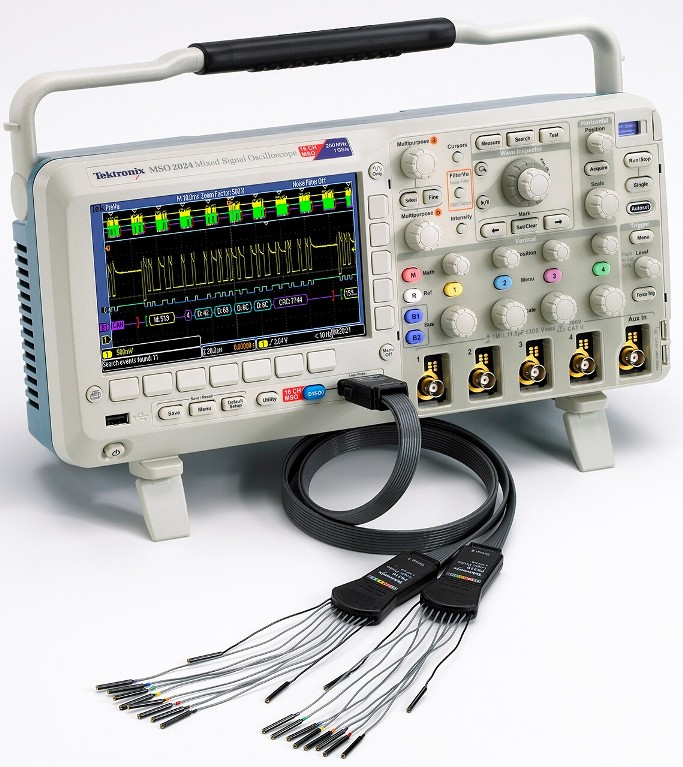
\includegraphics[scale=0.5]{dso.jpg}
\caption{un oscilloscopio}
\end{figure}

\newpage

\begin{tcolorbox}[breakable,colback=cyan,colframe=cyan]
\section*{Misurazione di valore efficace e frequenza}
\end{tcolorbox}

Impostazioni generatore di segnali :
\begin{itemize}
\item Segnale sinusoidale
\item Nessun offset
\item Ampiezza 1V
\item Frequenza 1Khz
\end{itemize}

Impostazioni oscilloscopio :
\begin{itemize}
\item Sensibilità orizzontale \(500  \mu S/div \)
\item Sensibilità verticale \(2 V/div\)
\end{itemize}

Collegamenti:
\begin{itemize}
\item Output del generatore di segnale collegato al CH1 dell'oscilloscopio con un cavo coassiale da \(50 \Omega\)  
\end{itemize}

Formula impiegata per il calcolo dell’incertezza: Modello probabilistico \[\bar{n} = \tfrac{1}{m}\sum_{k=1}^m n_k \]
\[s^2 (n_k)= \tfrac{1}{m-1}\sum_{k=1}^m (n_k - \bar{n})^2 \] 
\[s^2 (\bar{n}) = \tfrac{s^2 (n_k)}{m}\]

\subsection{Misurazione del valore efficace}

La misurazione della tensione di picco-picco permette di ricavare in maniera indiretta il valore efficace della tensione
\begin{itemize}
\item Lettura dell’ampiezza picco-picco \\ 
    \begin{tabular}{|r|l|l|l|l|}
     \hline
     \multicolumn{4}{|c|}{\(Vpp (mV)\)} \\
     \hline
     \(968,0\) & \(952,0\) & \(976,0\) & \(984,0\) \\
     \hline
   \end{tabular} \\ \\
Utilizzando la formula sotto specificata per il calcolo della media otteniamo:
\[\overline{Vpp}= 970,0 mV\]
\item Incertezza: \(\delta{}  Vpp= 6,83 mV\)
\item Valore efficace e incertezza \(Veff= \tfrac{Vpp}{\sqrt{2}} = 685,9 \pm 6,83 mV \)
\end{itemize}

\subsection{Misurazione di frequenza}
\begin{itemize}
\item \(T_1 = 1000 \mu s\) \(T_2 = 998 \mu s\) \(\overline{T} = 999 \pm 1 \mu s\)
\item \(f= 1,000 \pm 0,001 kHz\)
\end{itemize}

\subsection{Verifica con multimetro}
\begin{itemize}
\item \(Veff= 0,347 \pm 0,06 V \)
\item \(f= 1 \pm 0,010 kHz \)
\end{itemize}
\item Per verificarne la compatibilità : \(0,347 * \sqrt{2} = 0,49 V \approx 0,5\ V) rientra nell'incertezza 

\begin{tcolorbox}[breakable,colback=cyan,colframe=cyan]
\section*{Misurazione del tempo di salita}
\end{tcolorbox}

Impostazioni generatore di segnali :
\begin{itemize}
\item Segnale onda quadra
\item Nessun offset
\item Ampiezza 1V
\item Frequenza 1Khz
\end{itemize}

Impostazioni oscilloscopio :
\begin{itemize}
\item Sensibilità orizzontale \(10 nS/div \)
\item Sensibilità verticale \(2 V/div\)
\end{itemize}

Collegamenti:
\begin{itemize}
\item Output del generatore di segnale collegato al CH1 dell'oscilloscopio con un cavo coassiale da \(50 \Omega\)  
\end{itemize}

\subsection{ Misurazione 1}
\begin{itemize}
\item Il sistema in misura presenta un disadattamento d’impedenza il cui effetto `e quello di distorcere il fronte di salita del segnale. In queste condizioni il tempo di salita è \[ts1 = \tfrac{7,92+7,44+7,60+7,64+8,04}{5}ns = 7,73 \pm 0,11 ns\]
\item Misurazione in condizioni di adattamento \[ts_2 = \tfrac{7,28+7,16+7,36+7,24+6,84+7,56}{6}ns = 7,24 \pm 0,10 ns\] 
\item Tempo di salita introdotto dall’oscilloscopio a causa della sua banda passante \(tso=\tfrac{0.35}{B} = ns\) ;TODO
\item \(ts= \sqrt{ts_2^2 -tso^2} = ns\)
\end{itemize}

\subsection{Misurazione 2}

Collegamenti:
\begin{itemize}
\item Output del generatore di segnale collegato al CH1 dell'oscilloscopio con due cavi coassiali BNC-coccodrilli da \(50 \Omega\) intramezzati da una resistenza da \(1 K\Omega\) \\
Lunghezza cavi complessiva \(\approx 1 m\) 
\end{itemize}


\begin{enumerate}
\item Frequenza del polo ed effetto sulla misura del tempo di salita
  \begin{itemize}
    \item Capacità totale \(Ctot = C_{cavo} + C_{osci} = 100 pF + 13 pF = 113 pF\) \\ La capacità del cavo ci è stata fornita come valore approssimato quindi non è possibile risalire all'incertezza
    \item Resistenza del generatore ``modificato'' \(Rg= 1050 \Omega\)
    \item Frequenza polo \[fp = \tfrac{1}{2\pi \cdot Rg \cdot Ctot} = \tfrac{1}{2\pi \cdot 1050\Omega \cdot 113pF}kHz = 1,34\cdot10^3 kHz \]
    \item Tempo di salita dovuto al polo \(tsp= 0.35/fp = 261 ns\)
    \item Verifica sperimentale \[tsp_m = \tfrac{235+234+230+227+226}{5} ns = 230,4 \pm 1,54 ns\]
    \end{itemize}

\item Per ridurre questo effetto sistematico utilizziamo la sonda compensata al posto del cavo coassiale
 \begin{itemize}
 \item  \(C_s=\tfrac{R_{osci}\cdotC_{osci}}{R_s}= \tfrac{1*10^{12}\Omega\cdot13 pF}{9\cdot10^{12}\Omega} = 1,44 pF\)
 \item \(C_{tot}= C_{cavo}+C_{sonda}+C_{osci} = (1,44 +13 +100)pF = 114,44 pF\)
 \item Frequenza polo \(fp' = \tfrac{1}{2\pi\cdot114,44\cdot10^{-12}F} = 1,33 * 10^6 Hz\)
 \item Nuovo tempo di salita atteso \(tsp'= \tfrac{0,35}{fp'} = \tfrac{0,35}{1,33\cdot10^6 Hz}= 263,2 ns\)
 \item \(tsp'= \tfrac{246+257+245+215+252+259+260+261}{8}ns = 249,37 \pm 5,38 ns\)
 \end{itemize}
\end{enumerate}



\begin{tcolorbox}[breakable,colback=cyan,colframe=cyan]
\section*{Aliasing}
\end{tcolorbox}

Impostazioni generatore di segnali :
\begin{itemize}
\item Segnale sinusoidale
\item Nessun offset
\item Ampiezza 1V
\item Frequenza 100Khz
\end{itemize}

Impostazioni oscilloscopio :
\begin{itemize}
\item Sensibilità verticale \(2 V/div\)
\item Sensibilità orizzontale \(2,5 \muS/div \) 
\item Calcolo frequenza di campionamento minima \(fc \geq 2B = 200 kHz\)
\item Calcolo frequenza di campionamento oscilloscopio \(f_{co}=\tfrac{250}{vs}= 100 MHz\)
\end{itemize}

Collegamenti:
\begin{itemize}
\item Output del generatore di segnale collegato al CH1 dell'oscilloscopio con un cavo coassiale da \(50 \Omega\)  
\end{itemize}


\subsection{Aliasing percettivo}
 \begin{enumerate}
  \item Abbiamo ridotto la velocità di scansione
  \item Velocità di scansione tale per cui la frequenza vale \(fco= 1 MHz\)
  \item Abbiamo impostato lo strumento per la visualizzazione a punti
  \item Abbiamo modificato la frequenza del generatore a \(99,9 kHz\) e osserviamo che il segnale non è più sinusoidale per effetto dell'aliasing. \\ A \(99 KHz\) per effetto dell'aliasing percettivo ci sembra di vedere due sinusoidi sfasate 
 \end{enumerate}

;TODO FOTO

\subsection{Effetto dell’aliasing nel dominio del tempo}
 \begin{enumerate}
  \item Abbiamo impostato la frequenza del generatore di segnali a \(fg=100.1 kHz\)
  \item Abbiamo ridotto la frequenza di scansione fino ad avere una frequenza di campionamento di \(fco=100 kHz\) Abbiamo misurato la frequenza del segnale osservato \(fs= 102,2 kHz\)
  \item Abbiamo portato la frequenza del generatore di segnali a \(fg=100kHz\)
  \item FOTO
\end{enumerate}


\begin{tcolorbox}[breakable,colback=cyan,colframe=cyan]
\section*{Rilevazione sincrona di segnali}
\end{tcolorbox}


\subsection{Operazioni preliminari}
 \begin{enumerate}
  \item circuito
  \item generatori regolati come
   \begin{itemize}
     \item GEN1 Segnale sinusoidale, frequenza 480 Hz, Vp=2V
     \item GEN2 Segnale sinusoidale, ampiezza 1V, senza offset, frequenza 2kHz
   \end{itemize}
  \item Segnale del canale 1 con oscilloscopio sincronizzato sul canale 1 e poi sul canale 2

FOTO

\subsection{Misurazione}
  \item Oscilloscopio sincronizzato sul canale 2 con l'opzione media
  \item Abbiamo modificato il segnale di disturbo e il numero di medie
  \item Effetto media quando l'oscilloscopio è sincronizzato sul canale 1
 \end{enumerate}

\noindent \LaTeX

\end{document}






